% chktex-file 29
% chktex-file 13
\documentclass{report}
\usepackage{setspace}
\usepackage[a4paper, total={7in, 9in}]{geometry}
\usepackage[fleqn]{amsmath}
\usepackage{empheq}
\usepackage{amssymb}
\usepackage{amsthm}
\usepackage{gensymb}
\usepackage[fleqn]{cases}
\usepackage{multicol}
\usepackage{color}
\usepackage{stix}
\usepackage{chngcntr}
\usepackage{tikz}
\usetikzlibrary{calc,matrix}

\counterwithout{equation}{chapter}
\setlength{\columnseprule}{1pt}
\setlength{\columnsep}{24pt}
\setcounter{chapter}{11}
\hfuzz=100pt

\newtheorem{theorem}{Theorem}

\begin{document}
\newcommand{\sol}[1]{

    \noindent \textbf{Sol.}
}
\begin{titlepage}
    \raggedleft{}
    \rule{1pt}{\textheight}
    \hspace{0.02\textwidth}
    \parbox[b]{0.75\textwidth}{

    {\Huge\bfseries Solution Book of \\[0.5\baselineskip] Mathematic}\\[2\baselineskip]
    {\large\textit{Ssnior 2 Part I}}\\[4\baselineskip]
    {\Large\textsc{MELVIN CHIA}}

    \vspace{0.5\textheight}

    {\noindent Written on 9 October 2022}\\[\baselineskip]
    }

\end{titlepage}

\doublespacing{}
\tableofcontents
\singlespacing{}
\newpage

\begin{multicols}{2}
    \subsection{Exercise 14.4}
    Calculate the following products (Question 1 to 8):
    \begin{enumerate}
        \item $\begin{bmatrix}
                      1 & 2 & 3
                  \end{bmatrix}\begin{bmatrix}
                      1 \\
                      2 \\
                      3
                  \end{bmatrix}$
              \sol{}
              \begin{flalign*}
                   & \begin{bmatrix}
                         1 & 2 & 3
                     \end{bmatrix}\begin{bmatrix}
                                      1 \\
                                      2 \\
                                      3
                                  \end{bmatrix} \\
                   & = \begin{bmatrix}
                           1(1) + 2(2) + 3(3)
                       \end{bmatrix}              \\
                   & = \begin{bmatrix}
                           14
                       \end{bmatrix}
              \end{flalign*}
        \item $\begin{bmatrix}
                      1 \\
                      2 \\
                      3
                  \end{bmatrix}\begin{bmatrix}
                      1 & 2 & 3
                  \end{bmatrix}$
              \sol{}
              \begin{flalign*}
                   & \begin{bmatrix}
                         1 \\
                         2 \\
                         3
                     \end{bmatrix}\begin{bmatrix}
                                      1 & 2 & 3
                                  \end{bmatrix}    \\
                   & = \begin{bmatrix}
                           1 & 2 & 3 \\
                           2 & 4 & 6 \\
                           3 & 6 & 9
                       \end{bmatrix}
              \end{flalign*}
        \item $\begin{bmatrix}
                      2 & -3 \\
                      1 & 5
                  \end{bmatrix}\begin{bmatrix}
                      1 & 0 \\
                      0 & 1
                  \end{bmatrix}$
              \sol{}
              \begin{flalign*}
                   & \begin{bmatrix}
                         2 & -3 \\
                         1 & 5
                     \end{bmatrix}\begin{bmatrix}
                                      1 & 0 \\
                                      0 & 1
                                  \end{bmatrix}       \\
                   & = \begin{bmatrix}
                           2(1) + (-3)(0) & 2(0) + (-3)(1) \\
                           1(1) + 5(0)    & 1(0) + 5(1)
                       \end{bmatrix} \\
                   & = \begin{bmatrix}
                           2 & -3 \\
                           1 & 5
                       \end{bmatrix}
              \end{flalign*}
        \item $\begin{bmatrix}
                      -6 & -4 & 2  \\
                      7  & 8  & -5
                  \end{bmatrix}\begin{bmatrix}
                      1 & 2 & 3
                  \end{bmatrix}$
              \sol{}
              \begin{flalign*}
                   & \begin{bmatrix}
                         -6 & -4 & 2  \\
                         7  & 8  & -5
                     \end{bmatrix}\begin{bmatrix}
                                      1 & 2 & 3
                                  \end{bmatrix} \\
                   & = \begin{bmatrix}
                           -6(1) + (-4)(2) + 2(3) \\
                           7(1) + 8(2) + (-5)(3)
                       \end{bmatrix}    \\
                   & = \begin{bmatrix}
                           -8 \\
                           8
                       \end{bmatrix}
              \end{flalign*}
        \item $\begin{bmatrix}
                      2 & 3 & 4 \\
                      0 & 1 & 2
                  \end{bmatrix}\begin{bmatrix}
                      2 & 0 \\
                      3 & 1 \\
                      4 & 2
                  \end{bmatrix}$
              \sol{}
              \begin{flalign*}
                   & \begin{bmatrix}
                         2 & 3 & 4 \\
                         0 & 1 & 2
                     \end{bmatrix}\begin{bmatrix}
                                      2 & 0 \\
                                      3 & 1 \\
                                      4 & 2
                                  \end{bmatrix}    \\
                   & = \begin{bmatrix}
                           2(2) + 3(3) + 4(4) & 2(0) + 3(1) + 4(2) \\
                           0(2) + 1(3) + 2(4) & 0(0) + 1(1) + 2(2)
                       \end{bmatrix} \\
                   & = \begin{bmatrix}
                           27 & 11 \\
                           11 & 5
                       \end{bmatrix}
              \end{flalign*}
        \item $\begin{bmatrix}
                      6 & 4  & 2 \\
                      5 & -2 & 0 \\
                      0 & 3  & 1
                  \end{bmatrix}\begin{bmatrix}
                      5 \\
                      2 \\
                      3
                  \end{bmatrix}$
              \sol{}
              \begin{flalign*}
                   & \begin{bmatrix}
                         6 & 4  & 2 \\
                         5 & -2 & 0 \\
                         0 & 3  & 1
                     \end{bmatrix}\begin{bmatrix}
                                      5 \\
                                      2 \\
                                      3
                                  \end{bmatrix}          \\
                   & = \begin{bmatrix}
                           6(5) + 4(2) + 2(3)    \\
                           5(5) + (-2)(2) + 0(3) \\
                           0(5) + 3(2) + 1(3)
                       \end{bmatrix} \\
                   & = \begin{bmatrix}
                           44 \\
                           21 \\
                           9
                       \end{bmatrix}
              \end{flalign*}
        \item $\begin{bmatrix}
                      0 & 1 & 0 \\
                      1 & 0 & 0 \\
                      0 & 0 & 1
                  \end{bmatrix}\begin{bmatrix}
                      0 & 1 & 0 \\
                      1 & 0 & 0 \\
                      0 & 0 & 1
                  \end{bmatrix}$
              \sol{}
              \begin{flalign*}
                   & \begin{bmatrix}
                         0 & 1 & 0 \\
                         1 & 0 & 0 \\
                         0 & 0 & 1
                     \end{bmatrix}\begin{bmatrix}
                                      0 & 1 & 0 \\
                                      1 & 0 & 0 \\
                                      0 & 0 & 1
                                  \end{bmatrix}                           \\
                   & = \left[\begin{smallmatrix}
                                     0(0) + 1(1) + 0(0) & 0(1) + 1(0) + 0(0) & 0(0) + 1(0) + 0(1) \\
                                     1(0) + 0(1) + 0(0) & 1(1) + 0(0) + 0(0) & 1(0) + 0(0) + 0(1) \\
                                     0(0) + 0(1) + 1(0) & 0(1) + 0(0) + 1(0) & 0(0) + 0(0) + 1(1)
                                 \end{smallmatrix}\right] \\
                   & = \begin{bmatrix}
                           1 & 0 & 0 \\
                           0 & 1 & 0 \\
                           0 & 0 & 1
                       \end{bmatrix}
              \end{flalign*}
        \item $\begin{bmatrix}
                      1  & -1 & 1  \\
                      -3 & 2  & -1 \\
                      -2 & 1  & 0
                  \end{bmatrix}\begin{bmatrix}
                      1 & 2 & 3 \\
                      2 & 4 & 6 \\
                      1 & 2 & 3 \\
                  \end{bmatrix}$
              \sol{}
              \begin{flalign*}
                   & \begin{bmatrix}
                         1  & -1 & 1  \\
                         -3 & 2  & -1 \\
                         -2 & 1  & 0
                     \end{bmatrix}\begin{bmatrix}
                                      1 & 2 & 3 \\
                                      2 & 4 & 6 \\
                                      1 & 2 & 3
                                  \end{bmatrix}                     \\
                   & = \left[\begin{smallmatrix}
                                     1 + (-2) + 1     & 2 + (-4) + 2     & 3 + (-6) + 3     \\
                                     (-3) + 4 + (-1) & (-6) + 8 + (-2) & (-9) + 12 + (-3) \\
                                     (-2) + 2 + 0       & (-4) + 4 + 0       & (-6) + 6 + 0
                                 \end{smallmatrix}\right] \\
                   & = \begin{bmatrix}
                           0 & 0 & 0 \\
                           0 & 0 & 0 \\
                           0 & 0 & 0
                       \end{bmatrix}
              \end{flalign*}
    \end{enumerate}

    \section{Determinants}

    The determinant of an n-order matrix $A = {(a_{ij})}_{n\times n}$ is denoted as
    $\det(A)$. When $n \leq 2$, the deternimant can also be denoted as $|A|$. The
    determinant is a value.

    When $n = 1$, the determinant is the value of the only element in the matrix.

    \subsection*{Determinant of a 2x2 matrix}

    For a 2x2 matrix, the determinant is defined as:
    \begin{flalign*}
        \det(A) = \begin{vmatrix}
                      a & b \\
                      c & d
                  \end{vmatrix} = ad - bc
    \end{flalign*}

    \subsection{Practice 4}
    Find the value of the following determinants.
    \begin{enumerate}
        \item $\begin{vmatrix}
                      2 & -3 \\
                      5 & 7
                  \end{vmatrix}$
              \sol{}
              \begin{flalign*}
                   & \begin{vmatrix}
                         2 & -3 \\
                         5 & 7
                     \end{vmatrix}   \\
                   & = 2(7) - (-3)(5) \\
                   & = 14 + 15        \\
                   & = 29
              \end{flalign*}
        \item $\begin{vmatrix}
                      -6 & -7 \\
                      -8 & -9
                  \end{vmatrix}$
              \sol{}
              \begin{flalign*}
                   & \begin{vmatrix}
                         -6 & -7 \\
                         -8 & -9
                     \end{vmatrix}        \\
                   & = (-6)(-9) - (-7)(-8) \\
                   & = 54 - 56             \\
                   & = -2
              \end{flalign*}
        \item $\begin{vmatrix}
                      12  & -20 \\
                      -21 & 35
                  \end{vmatrix}$
              \sol{}
              \begin{flalign*}
                   & \begin{vmatrix}
                         12  & -20 \\
                         -21 & 35
                     \end{vmatrix}        \\
                   & = 12(35) - (-20)(-21) \\
                   & = 420 - 420           \\
                   & = 0
              \end{flalign*}
    \end{enumerate}

    \subsection*{Determinant of a 3x3 matrix}

    For a 3x3 matrix, the determinant is defined as:
    \begin{flalign*}
        \det(A) & = \begin{vmatrix}
                        a_1 & b_1 & c_1 \\
                        a_2 & b_2 & c_2 \\
                        a_3 & b_3 & c_3
                    \end{vmatrix}                       \\
                & = a_1\begin{vmatrix}
                           b_2 & c_2 \\
                           b_3 & c_3
                       \end{vmatrix} - b_1\begin{vmatrix}
                                              a_2 & c_2 \\
                                              a_3 & c_3
                                          \end{vmatrix} + c_1\begin{vmatrix}
                                                                 a_2 & b_2 \\
                                                                 a_3 & b_3
                                                             \end{vmatrix}   \\
                & = a_1b_2c_3 + b_1c_2a_3 + c_1a_2b_3 - a_3b_2c_1 - b_3c_2a_1 \\
                & \ \ \ \ - c_3a_2b_1
    \end{flalign*}

    A 3x3 matrix can be expanded using the Sarrus method. The Sarrus method is
    defined as:

    \begin{center}
        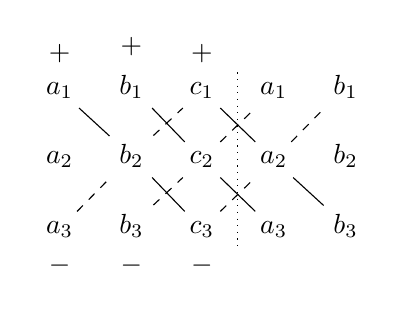
\begin{tikzpicture}
            \matrix [%
                matrix of math nodes,
                column sep=1em,
                row sep=1em
            ] (sarrus) {%
                a_1 & b_1 & c_1 & a_1 & b_1 \\
                a_2 & b_2 & c_2 & a_2 & b_2 \\
                a_3 & b_3 & c_3 & a_3 & b_3 \\
            };

            \path ($(sarrus-1-3.north east)+(0.5em,0)$) edge[dotted] ($(sarrus-3-3.south east)+(0.5em,0)$)
            (sarrus-1-1)                          edge         (sarrus-2-2)
            (sarrus-2-2)                          edge         (sarrus-3-3)
            (sarrus-1-2)                          edge         (sarrus-2-3)
            (sarrus-2-3)                          edge         (sarrus-3-4)
            (sarrus-1-3)                          edge         (sarrus-2-4)
            (sarrus-2-4)                          edge         (sarrus-3-5)
            (sarrus-3-1)                          edge[dashed] (sarrus-2-2)
            (sarrus-2-2)                          edge[dashed] (sarrus-1-3)
            (sarrus-3-2)                          edge[dashed] (sarrus-2-3)
            (sarrus-2-3)                          edge[dashed] (sarrus-1-4)
            (sarrus-3-3)                          edge[dashed] (sarrus-2-4)
            (sarrus-2-4)                          edge[dashed] (sarrus-1-5);

            \foreach \c in {1,2,3} {\node[anchor=south] at (sarrus-1-\c.north) {$+$};};
            \foreach \c in {1,2,3} {\node[anchor=north] at (sarrus-3-\c.south) {$-$};};
        \end{tikzpicture}
    \end{center}

    Note that the Sarrus method is only applicable to 3x3 matrices.

    \subsection{Practice 5}

    Calculate the value of the following determinants.

    \begin{enumerate}
        \item $\begin{vmatrix}
                      1 & 5 & 1 \\
                      1 & 6 & 3 \\
                      9 & 8 & 9
                  \end{vmatrix}$
              \sol{}

              \begin{center}
                  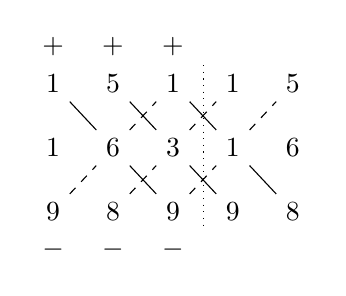
\begin{tikzpicture}
                      \matrix [%
                          matrix of math nodes,
                          column sep=1em,
                          row sep=1em
                      ] (sarrus) {%
                          1 & 5 & 1 & 1 & 5 \\
                          1 & 6 & 3 & 1 & 6 \\
                          9 & 8 & 9 & 9 & 8 \\
                      };

                      \path ($(sarrus-1-3.north east)+(0.5em,0)$) edge[dotted] ($(sarrus-3-3.south east)+(0.5em,0)$)
                      (sarrus-1-1)                          edge         (sarrus-2-2)
                      (sarrus-2-2)                          edge         (sarrus-3-3)
                      (sarrus-1-2)                          edge         (sarrus-2-3)
                      (sarrus-2-3)                          edge         (sarrus-3-4)
                      (sarrus-1-3)                          edge         (sarrus-2-4)
                      (sarrus-2-4)                          edge         (sarrus-3-5)
                      (sarrus-3-1)                          edge[dashed] (sarrus-2-2)
                      (sarrus-2-2)                          edge[dashed] (sarrus-1-3)
                      (sarrus-3-2)                          edge[dashed] (sarrus-2-3)
                      (sarrus-2-3)                          edge[dashed] (sarrus-1-4)
                      (sarrus-3-3)                          edge[dashed] (sarrus-2-4)
                      (sarrus-2-4)                          edge[dashed] (sarrus-1-5);

                      \foreach \c in {1,2,3} {\node[anchor=south] at (sarrus-1-\c.north) {$+$};};
                      \foreach \c in {1,2,3} {\node[anchor=north] at (sarrus-3-\c.south) {$-$};};
                  \end{tikzpicture}
              \end{center}
              \begin{flalign*}
                  \begin{vmatrix}
                      1 & 5 & 1 \\
                      1 & 6 & 3 \\
                      9 & 8 & 9
                  \end{vmatrix} & = 54 + 135 + 8 - 54 - 24 - 45 \\
                                                 & = 74
              \end{flalign*}
        \item $\begin{vmatrix}
                      3 & 1  & -2 \\
                      0 & -1 & 1  \\
                      4 & 2  & 5
                  \end{vmatrix}$
              \sol{}

              \begin{center}
                  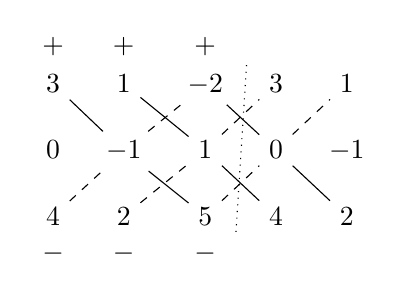
\begin{tikzpicture}
                      \matrix [%
                          matrix of math nodes,
                          column sep=1em,
                          row sep=1em
                      ] (sarrus) {%
                          3 & 1  & -2 & 3 & 1  \\
                          0 & -1 & 1  & 0 & -1 \\
                          4 & 2  & 5  & 4 & 2  \\
                      };

                      \path ($(sarrus-1-3.north east)+(0.5em,0)$) edge[dotted] ($(sarrus-3-3.south east)+(0.5em,0)$)
                      (sarrus-1-1)                          edge         (sarrus-2-2)
                      (sarrus-2-2)                          edge         (sarrus-3-3)
                      (sarrus-1-2)                          edge         (sarrus-2-3)
                      (sarrus-2-3)                          edge         (sarrus-3-4)
                      (sarrus-1-3)                          edge         (sarrus-2-4)
                      (sarrus-2-4)                          edge         (sarrus-3-5)
                      (sarrus-3-1)                          edge[dashed] (sarrus-2-2)
                      (sarrus-2-2)                          edge[dashed] (sarrus-1-3)
                      (sarrus-3-2)                          edge[dashed] (sarrus-2-3)
                      (sarrus-2-3)                          edge[dashed] (sarrus-1-4)
                      (sarrus-3-3)                          edge[dashed] (sarrus-2-4)
                      (sarrus-2-4)                          edge[dashed] (sarrus-1-5);

                      \foreach \c in {1,2,3} {\node[anchor=south] at (sarrus-1-\c.north) {$+$};};
                      \foreach \c in {1,2,3} {\node[anchor=north] at (sarrus-3-\c.south) {$-$};};
                  \end{tikzpicture}
              \end{center}
              \begin{flalign*}
                  \begin{vmatrix}
                      3 & 1  & -2 \\
                      0 & -1 & 1  \\
                      4 & 2  & 5
                  \end{vmatrix} & = -15 + 4 - 0 - 8 - 6 - 0 \\
                                                    & = -25
              \end{flalign*}
    \end{enumerate}
    \subsection*{Minor and Cofactor}

    The minor of an element in a matrix is the determinant of the matrix obtained
    by deleting the row and column containing the element. Take $\begin{vmatrix}
            a_1 & a_2 & a_3 \\ b_1 & b_2 & b_3 \\ c_1 & c_2 & c_3 \end{vmatrix}$ as an example. The minor of $a_1$ is
    $\begin{vmatrix} b_2 & c_2 \\ b_3 & c_3 \end{vmatrix}$, the minor of $c_2$ is $\begin{vmatrix} a_1 & b_1 \\ a_3 & b_3 \end{vmatrix}$, and so on.

    The cofactor of an element in a matrix is the minor of the element multiplied
    by ${(-1)}^{i+j}$, where $i$ and $j$ are the row and column indices of the
    element. The cofactor of $a_1$ is ${(-1)}^{1+1}\begin{vmatrix} b_2 & c_2 \\ b_3 & c_3 \end{vmatrix}$, the cofactor of $c_2$ is ${(-1)}^{3+2}\begin{vmatrix} a_1 & b_1 \\ a_3 & b_3 \end{vmatrix}$, and so on.

    Let $A_1, B_1, C_1$ are the cofactors of $a_1, b_1, c_1$ respectively. Then

    \begin{flalign*}
        A_1 & = (-1)^{1+1}\begin{vmatrix} b_2 & c_2 \\ b_3 & c_3 \end{vmatrix} = \begin{vmatrix} b_2 & c_2 \\ b_3 & c_3 \end{vmatrix}  \\
        B_1 & = (-1)^{1+2}\begin{vmatrix} a_2 & c_2 \\ a_3 & c_3 \end{vmatrix} = -\begin{vmatrix} a_2 & c_2 \\ a_3 & c_3 \end{vmatrix} \\
        C_1 & = (-1)^{1+3}\begin{vmatrix} a_2 & b_2 \\ a_3 & b_3 \end{vmatrix} = \begin{vmatrix} a_2 & b_2 \\ a_3 & b_3 \end{vmatrix}
    \end{flalign*}

    Thus,
    \[|A| =  a_1A_1 + a_2B_1 + a_3C_1\]

    That is, the value of the determinant is the elements of the first row
    multiplied by the cofactors of the elements of the first row.

    The sign of the cofactor is determined by the sum of the row and column indices
    of the element. If the sum is even, the cofactor is positive; if the sum is
    odd, the cofactor is negative.\newline\newline \noindent Generally, a 3x3
    determinant has the following theorem:

    \begin{theorem}
        The determinant of a 3x3 matrix is the sum of the elements of any row or
        column multiplied by the cofactors of the elements of that row or column.
    \end{theorem}

    That is, we can use the cofactor expansion to calculate the determinant of a
    3x3 matrix.

    \begin{flalign*}
        \begin{vmatrix}A\end{vmatrix} & = a_1A_1 + b_1B_1 + c_1C_1 \\
                                      & = a_2B_2 + b_2B_2 + c_2C_2 \\
                                      & = a_3C_3 + b_3C_3 + c_3C_3 \\
                                      & = a_1A_1 + a_2A_2 + a_3A_3 \\
                                      & = b_1B_1 + b_2B_2 + b_3B_3 \\
                                      & = c_1C_1 + c_2C_2 + c_3C_3
    \end{flalign*}

    The determinant of any order matrix can also be calculated by the cofactor
    expansion.

    \begin{theorem}
        The product of the elements of any row or column and the cofactor of corresponding elements of another row or column of a determinant is 0.
    \end{theorem}
    For example, the product of the elements of the second row and the corresponding element of the cofactor of first row of the determinant is 0. That is,
    \begin{flalign*}
         & a_2B_1 + b_2B_1 + c_2C_1                                                                                                                                                      \\
         & = a_2\begin{vmatrix} b_2 & c_2 \\ b_3 & c_3 \end{vmatrix} - b_2\begin{vmatrix} a_2 & c_2 \\ a_3 & c_3 \end{vmatrix} + c_2\begin{vmatrix} a_2 & b_2 \\ a_3 & b_3 \end{vmatrix} \\
         & = a_2b_2c_3 + a_2b_3c_2 - a_2b_2c_3 + a_3b_2c_2 + a_2b_3c_2 - a_3b_2c_2                                                                                                       \\
         & = 0
    \end{flalign*}

    \subsection{Practice 6}
    Find the value of the following 3x3 determinants.

    \begin{enumerate}
        \item $\begin{vmatrix} 4 & -2 & 1 \\ 1 & -3 & 0 \\ 2 & 7 & -1 \end{vmatrix}$
              \sol{}
              \begin{flalign*}
                   & \begin{vmatrix} 4 & -2 & 1 \\ 1 & -3 & 0 \\ 2 & 7 & -1 \end{vmatrix}                                                                             \\
                   & = 4\begin{vmatrix} - 3 & 0 \\ 7 & -1 \end{vmatrix} - \begin{vmatrix} -2 & 1 \\ 7 & -1 \end{vmatrix} + 2 \begin{vmatrix} -2 & 1 \\ -3 & 0 \end{vmatrix} \\
                   & = 4(3 - 0) - (2 - 7) + 2(0 + 3)                                                                                                                        \\
                   & = 12 + 5 + 6                                                                                                                                           \\
                   & = 23
              \end{flalign*}

        \item $\begin{vmatrix} 5 & -4 & 2 \\ 1 & 0 & -3 \\ 1 & -1 & 2 \end{vmatrix}$
              \sol{}
              \begin{flalign*}
                   & \begin{vmatrix} 5 & -4 & 2 \\ 1 & 0 & -3 \\ 1 & -1 & 2 \end{vmatrix}                                                                          \\
                   & = 5\begin{vmatrix} 0 & -3 \\ -1 & 2 \end{vmatrix} - \begin{vmatrix} -4 & 2 \\ -1 & 2 \end{vmatrix} + \begin{vmatrix} -4 & 2 \\ 0 & -3 \end{vmatrix} \\
                   & = 5(0 - 3) - (-8 + 2) + (12 + 0)                                                                                                                    \\
                   & = -15 + 6 + 12                                                                                                                                      \\
                   & = 3
              \end{flalign*}

        \item $\begin{vmatrix} 2 & 0 & 1 \\ 0 & 2 & 0 \\ 2 & 0 & -1 \end{vmatrix}$
              \sol{}
              \begin{flalign*}
                   & \begin{vmatrix} 2 & 0 & 1 \\ 0 & 2 & 0 \\ 2 & 0 & -1 \end{vmatrix}                                                                          \\
                   & = 2\begin{vmatrix} 2 & 0 \\ 0 & -1 \end{vmatrix} - 0\begin{vmatrix} 0 & 1 \\ 0 & -1 \end{vmatrix} + 2\begin{vmatrix} 0 & 1 \\ 2 & 0 \end{vmatrix} \\
                   & = 2(-2 - 0) + 2(-2)                                                                                                                               \\
                   & = -4 - 4                                                                                                                                          \\
                   & = -8
              \end{flalign*}
    \end{enumerate}

    \subsection{Exercise 14.5a}

    Find the value of the following determinants.

    \begin{enumerate}
        \item $\begin{vmatrix} 3 & 2 \\ 1 & -4 \end{vmatrix}$
              \sol{}
              \begin{flalign*}
                   & \begin{vmatrix} 3 & 2 \\ 1 & -4 \end{vmatrix} \\
                   & = 3(-4) - 2(1)                                \\
                   & = -12 - 2                                     \\
                   & = -14
              \end{flalign*}

        \item $\begin{vmatrix} 35 & -2 \\ -11 & 5 \end{vmatrix}$
              \sol{}
              \begin{flalign*}
                   & \begin{vmatrix} 35 & -2 \\ -11 & 5 \end{vmatrix} \\
                   & = 35(5) - (-2)(-11)                              \\
                   & = 175 - 22                                       \\
                   & = 153
              \end{flalign*}

        \item $\begin{vmatrix} 1 & a \\ -a & 1 \end{vmatrix}$
              \sol{}
              \begin{flalign*}
                   & \begin{vmatrix} 1 & a \\ -a & 1 \end{vmatrix} \\
                   & = 1(1) - a(-a)                                \\
                   & = 1 + a^2                                     \\
              \end{flalign*}

        \item $\begin{vmatrix} \sin{x} & -\cos{x} \\ \cos{x} & \sin{x} \end{vmatrix}$
              \sol{}
              \begin{flalign*}
                   & \begin{vmatrix} \sin{x} & -\cos{x} \\ \cos{x} & \sin{x} \end{vmatrix} \\
                   & = \sin{x}\sin{x} - (-\cos{x})(\cos{x})                                \\
                   & = \sin^2{x} + \cos^2{x}                                               \\
                   & = 1
              \end{flalign*}

        \item $\begin{vmatrix} 1 & -2 & 3 \\ 2 & 3 & -4 \\ 3 & -2 & 5 \end{vmatrix}$
              \sol{}
              \begin{flalign*}
                   & \begin{vmatrix} 1 & -2 & 3 \\ 2 & 3 & -4 \\ 3 & -2 & 5 \end{vmatrix}                                                                            \\
                   & = 1\begin{vmatrix} 3 & -4 \\ -2 & 5 \end{vmatrix} - 2\begin{vmatrix} -2 & 3 \\ -2 & 5 \end{vmatrix} + 3\begin{vmatrix} -2 & 3 \\ 3 & -4 \end{vmatrix} \\
                   & = 1(15 - 8) - 2(-10 + 6) + 3(8 - 9)                                                                                                                   \\
                   & = 7 + 8 - 3                                                                                                                                           \\
                   & = 12                                                                                                                                                  \\
              \end{flalign*}

        \item $\begin{vmatrix} 1 & -3 & 4 \\ 2 & 0 & -5 \\ 3 & -1 & 7 \end{vmatrix}$
              \sol{}
              \begin{flalign*}
                   & \begin{vmatrix} 1 & -3 & 4 \\ 2 & 0 & -5 \\ 3 & -1 & 7 \end{vmatrix}                                                                           \\
                   & = \begin{vmatrix} 0 & -5 \\ -1 & 7 \end{vmatrix} - 2\begin{vmatrix} -3 & 4 \\ -1 & 7 \end{vmatrix} + 3\begin{vmatrix} -3 & 4 \\ 0 & -5 \end{vmatrix} \\
                   & = (0 - 5) - 2(-21 + 4) + 3(15 - 0)                                                                                                                   \\
                   & = -5 + 34 + 45                                                                                                                                       \\
                   & = 74
              \end{flalign*}

        \item $\begin{vmatrix} -1 & 3 & -2 \\ -3 & 2 & 0 \\ 4 & 0 & 5 \end{vmatrix}$
              \sol{}
              \begin{flalign*}
                   & \begin{vmatrix} -1 & 3 & -2 \\ -3 & 2 & 0 \\ 4 & 0 & 5 \end{vmatrix}                                                                        \\
                   & = -1\begin{vmatrix} 2 & 0 \\ 0 & 5 \end{vmatrix} + 3\begin{vmatrix} 3 & -2 \\ 0 & 5 \end{vmatrix} + 4\begin{vmatrix} 3 & -2 \\ 2 & 0 \end{vmatrix} \\
                   & = -1(10) + 3(-15 + 0) + 4(0 + 4)                                                                                                                   \\
                   & = -10 + 45 + 16                                                                                                                                    \\
                   & = 51
              \end{flalign*}

        \item $\begin{vmatrix} 0 & -q & -r \\ q & 0 & -s \\ r & s & 0 \end{vmatrix}$
              \sol{}
              \begin{flalign*}
                   & \begin{vmatrix} 0 & -q & -r \\ q & 0 & -s \\ r & s & 0 \end{vmatrix}                                                                           \\
                   & = 0\begin{vmatrix} 0 & -s \\ s & 0 \end{vmatrix} - q\begin{vmatrix} -q & -r \\ s & 0 \end{vmatrix} + r\begin{vmatrix} -q & -r \\ 0 & -s \end{vmatrix} \\
                   & = 0 - q(0 + sr) + r(0 + qs)                                                                                                                           \\
                   & = 0
              \end{flalign*}

        \item $\begin{vmatrix} p & -q & r \\ q & r & -s \\ -r & s & p \end{vmatrix}$
              \sol{}
              \begin{flalign*}
                   & \begin{vmatrix} p & -q & r \\ q & r & -s \\ -r & s & p \end{vmatrix}                                                                          \\
                   & = p\begin{vmatrix} r & -s \\ s & p \end{vmatrix} - q\begin{vmatrix} -q & r \\ s & p \end{vmatrix} + r\begin{vmatrix} -q & r \\ r & -s \end{vmatrix} \\
                   & = p(rp + s^2) -q(-qp - sr) - r(qs - r^2)                                                                                                            \\
                   & = rp^2 + p{s}^2 + q^2 p + qsr - qsr + r^3                                                                                                           \\
                   & = rp^2 + s^2p + q^2 p - r^3
              \end{flalign*}

        \item $\begin{vmatrix} 1 & x & a \\ 1 & y & b \\ 1 & z & c \end{vmatrix}$
              \sol{}
              \begin{flalign*}
                   & \begin{vmatrix} 1 & x & a \\ 1 & y & b \\ 1 & z & c \end{vmatrix}                                                                     \\
                   & = \begin{vmatrix} y & b \\ z & c \end{vmatrix} - \begin{vmatrix} x & a \\ z & c \end{vmatrix} + \begin{vmatrix} x & a \\ y & b \end{vmatrix} \\
                   & = (yc - bz) - (xc - az) + (xb - ay)                                                                                                          \\
                   & = bx + cy + az - cx - ay - bz
              \end{flalign*}
    \end{enumerate}
    \subsection*{Properties of Determinants}

    \setcounter{theorem}{0}

    \begin{theorem}
        The value of a determinant is the same as the value of its transpose, aka $|A| = |A'|$.
        \begin{flalign*}
             & \begin{vmatrix} a & b \\ c & d \end{vmatrix} = \begin{vmatrix} a & c \\ b & d \end{vmatrix}
        \end{flalign*}
    \end{theorem}
    \begin{theorem}
        Switching any two rows or columns of a determinants results in the opposite value.
        \begin{flalign*}
             & \begin{vmatrix} a_1 & b_1 & c_1 \\ a_2 & b_2 & c_2 \\ a_3 & b_3 & c_3 \end{vmatrix} = -\begin{vmatrix} a_1 & b_1 & c_1 \\ a_3 & b_3 & c_3 \\ a_2 & b_2 & c_2 \end{vmatrix}
        \end{flalign*}
    \end{theorem}

    \subsection{Practice 7}

    Given $\begin{vmatrix}
            a & b & c \\
            d & e & f \\
            g & h & i
        \end{vmatrix} = 10$, find $\begin{vmatrix}
            b & c & a \\
            e & f & d \\
            h & i & g
        \end{vmatrix}$.
    \sol{}
    \begin{flalign*}
        \begin{vmatrix}
            b & c & a \\
            e & f & d \\
            h & i & g
        \end{vmatrix}
         & = -\begin{vmatrix}
                  a & c & b \\
                  d & f & e \\
                  g & i & h
              \end{vmatrix} \\
         & = \begin{vmatrix}
                 a & b & c \\
                 d & e & f \\
                 g & h & i
             \end{vmatrix}  \\
         & = 10
    \end{flalign*}
    \begin{theorem}
        If two rows or cols of a determinant are identical, the value of the determinant is zero.
        \begin{flalign*}
             & \begin{vmatrix} a & b & c \\ a & b & c \\ d & e & f \end{vmatrix} = 0 \\
        \end{flalign*}
    \end{theorem}
    \begin{theorem}
        If all elements of a row (or column) of a determinant are multiplied by some scalar number k, the value of the new determinant is k times of the given determinant.
        \begin{flalign*}
             & \begin{vmatrix} a_1 & b_1 & c_1 \\ ka_2 & kb_2 & kc_2 \\ a_3 & b_3 & c_3 \end{vmatrix} = k\begin{vmatrix} a_1 & b_1 & c_1 \\ a_2 & b_2 & c_2 \\ a_3 & b_3 & c_3 \end{vmatrix}
        \end{flalign*}
    \end{theorem}

    \subsection{Practice 8}

    Using the properties of determinants, prove that $\begin{vmatrix}
            10  & -12 & 2  \\
            -15 & 18  & 3  \\
            5   & 6   & -1
        \end{vmatrix} = 180\begin{vmatrix}
            1  & -1 & 1  \\
            -1 & 1  & 1  \\
            1  & 1  & -1
        \end{vmatrix}$.
    \sol{}
    \begin{flalign*}
         & \begin{vmatrix} 10 & -12 & 2 \\ -15 & 18 & 3 \\ 5 & 6 & -1 \end{vmatrix} \\
         & = 5\times6\begin{vmatrix}
                         2  & -2 & 2  \\
                         -3 & 3  & 3  \\
                         1  & 1  & -1
                     \end{vmatrix}                                    \\
         & = 5\times6\times2\times3\times\begin{vmatrix}
                                             1  & -1 & 1  \\
                                             -1 & 1  & 1  \\
                                             1  & 1  & -1
                                         \end{vmatrix}                \\
         & = 180\begin{vmatrix}
                    1  & -1 & 1  \\
                    -1 & 1  & 1  \\
                    1  & 1  & -1
                \end{vmatrix}
    \end{flalign*}

    \begin{theorem}
        In a determinant each element in any row (or column) consists of the sum of two terms, then the determinant can be expressed as sum of two determinants of same order.
        \begin{flalign*}
             & \begin{vmatrix} a_1+d_1 & b_1 & c_1 \\ a_2+d_2 & b_2 & c_2 \\ a_3+d_3 & b_3 & c_3 \end{vmatrix} = \begin{vmatrix} a_1 & b_1 & c_1 \\ a_2 & b_2 & c_2 \\ a_3 & b_3 & c_3 \end{vmatrix} + \begin{vmatrix} d_1 & b_1 & c_1 \\ d_2 & b_2 & c_2 \\ d_3 & b_3 & c_3 \end{vmatrix}
        \end{flalign*}
    \end{theorem}
    \begin{theorem}
        If a determinant is obtained by adding a row or column multiplied by a some scalar number k to a different row or column, then the value of the new determinant is the same as the original determinant.
        \begin{flalign*}
             & \begin{vmatrix} a_1 & b_1 & c_1 \\ a_2 & b_2 & c_2 \\ a_3 & b_3 & c_3 \end{vmatrix} = \begin{vmatrix} a_1+ka_2 & b_1+kb_2 & c_1+kc_2 \\ a_2 & b_2 & c_2 \\ a_3 & b_3 & c_3 \end{vmatrix}
        \end{flalign*}
    \end{theorem}

    \subsection{Practice 9}

    Prove that $\begin{vmatrix}
            1 & 2 & 3 \\
            4 & 5 & 6 \\
            7 & 8 & 9
        \end{vmatrix} = 0$.
    \sol{}
    \begin{flalign*}
         & \begin{vmatrix} 1 & 2 & 3 \\ 4 & 5 & 6 \\ 7 & 8 & 9 \end{vmatrix}                                                            \\
         & = \begin{vmatrix} 1 & 2 & 3 \\ 3 & 3 & 3 \\ 6 & 6 & 6 \end{vmatrix}  & (\text{Adding row 1 multiplied by -1 to row 2 and 3}) \\
         & = 2\begin{vmatrix} 1 & 2 & 3 \\ 3 & 3 & 3 \\ 3 & 3 & 3 \end{vmatrix} & (\text{Theorem 4})                                    \\
         & = 0                                                                         & (\text{Theorem 3})
    \end{flalign*}

    \begin{theorem}
        The determinant of product of two matrices of equal size is equal to the product of determinants of each matrix, aka $|AB| = |A||B|$.
    \end{theorem}

    \subsection{Practice 10}

    Let $A = \begin{vmatrix}
            -2 & 1 \\
            4  & 3
        \end{vmatrix}$ and $B = \begin{vmatrix}
            1 & x \\
            2 & 3
        \end{vmatrix}$. Given that $|AB| = -18$, find $x$.
    \sol{}
    \begin{flalign*}
        \because\ |AB| = |A||B|      & = -18           \\
        \therefore\ \begin{vmatrix}
                        -2 & 1 \\
                        4  & 3
                    \end{vmatrix}\begin{vmatrix}
                                     1 & x \\
                                     2 & 3
                                 \end{vmatrix} & = -18 \\
        -2(3-2x)                     & = -18           \\
        3-2x                         & = 9             \\
        -2x                          & = 6             \\
        x                            & = -3
    \end{flalign*}

\end{multicols}
\end{document}